\documentclass{article}

% set font encoding for PDFLaTeX, XeLaTeX, or LuaTeX
\usepackage{ifxetex,ifluatex,amsmath}
\if\ifxetex T\else\ifluatex T\else F\fi\fi T%
  \usepackage{fontspec}
\else
  \usepackage[T1]{fontenc}
  \usepackage[utf8]{inputenc}
  \usepackage{lmodern}
\fi

\usepackage{hyperref}
%Import physics package
\usepackage{physics,mathtools}
%import syntax package
\usepackage{listings, listings-rust}
%Formats URL's
\usepackage{url}
%Draw stuff
\usepackage{tikz}
%For linking to images
\usepackage{caption}

\title{PWS/Meesterproef vloeistofdynamica}
\author{Wiebe Derksen and Daniël Visser}


\begin{document}
\maketitle
\thispagestyle{empty}
\hfil
\thanks{PWS begeleiders meneer Straatman en meneer Matena, expertbegeleider Aron Van Den Bogaard}
\newpage
\tableofcontents
\newpage
%Start van het PWS zelf
\section{Introduction}
People have been simulating liquids and gasses for decades using computers.
\newpage

\section{The Navier-Stokes equations}
The Navier Stokes equations are \cite{Navier Stokes compressible}:
\begin{equation}
%x-component
\begin{multlined}
\rho (\pdv{u}{t} + u \pdv{u}{x} + v \pdv{u}{y}+w\pdv{u}{z}) \\ = \rho g_{x}-\pdv{P}{x}+\pdv{x} \bqty{2\mu \pdv{u}{x} + \lambda div \vec{V}}\\ + \pdv{y} \bqty{\mu(\pdv{u}{y}+\pdv{v}{z})}+\pdv{z} \bqty{\mu (\pdv{u}{z}+\pdv{w}{x})}
\end{multlined}
\label{NSE-x}
\end{equation}

%y-component
\begin{equation}
\begin{split}
\rho(\pdv{v}{t}&+u\pdv{v}{x}+v\pdv{v}{y}+w\pdv{v}{z}) \\&=\rho g_{y} -\pdv{P}{y} +\pdv{x} \bqty{\mu(\pdv{u}{y}+\pdv{v}{x})}\\&+ \pdv{y} \bqty{2\mu \pdv{v}{y} + \lambda div\vec{V}} +\pdv{z} \bqty{\mu(\pdv{v}{z}+\pdv{w}{y})}
\end{split}
\label{NSE-y}
\end{equation}

%z-component
\begin{equation}
\begin{split}
\rho (\pdv{v}{t}& + u \pdv{w}{x} + v \pdv{w}{y} +  w \pdv{w}{x}) \\&= \rho g_{z} - \pdv{P}{z} + \pdv{x} \bqty{\mu(\pdv{u}{z}+\pdv{w}{x})}+\\ &\pdv{y}\bqty{\mu (\pdv{v}{z}+\pdv{w}{y})} +\pdv{x} 2\mu  \pdv{w}{y}+\lambda div \vec(V)
\label{NSE-z}
\end{split}
\end{equation}

\newpage
\section{What algorithms are feasible to implement?}
\subsection{Introduction to differential equations}
There are many algorithms to execute fluid simulations, each has its own advantages and disadvantages. In this chapter we will discuss these algorithms and their pro's and cons. 
\\

A differential equation can be solved either numerically or analytically. An analytical solution is a solution for the entire domain of the function. A numerical solution only gives an approximation for some discrete values.  Many differential equations are not analytically solvable, they have to be solved numerically. A numerical solution is often obtained using computers. \cite{What is discretization}




%Algorithms
\subsection{The algorithms}
In this section we will discuss some of the most used algorithms for solving the Navier-Stokes Equations, their advantages and disadvantages. 
%FDM
\subsubsection{Finite Difference Method(FDM)}
The Finite Difference Method(FDM) approximates the derivatives of a function using a truncated Taylor series. For a Taylor series around a point x=a the following formula applies. :\cite{Taylor series}:
\[f(x)=\sum_{i=0}^{\infty}\frac{f^{(i)}}{i!}(x-a)^{i}\]
A computer cannot keep computing forever. Therefore we have to use a truncated Taylor series. The truncated Taylor series unto i=3 is given by \cite{Taylor series approximation}
\[f(x)=f(a)+f'(a)(x-a)+\frac{f``(a)(x-a)^{2}}{2} + \frac{f^{(3)}(a)(x-a)^{3}}{6}+O(\Delta x)^{4}\]
$O(\Delta x) ^{4}$ are the truncated terms.\cite{Big O}. Using the above formula, we can calculate $f(x+\Delta x)$ by taking a=x\cite{quantstart FDM}
\begin{equation}f(x+\Delta x)=f(x)+f`(x)\Delta x + \frac{f``(x) (\Delta x)^{2}}{2}+ \frac{f^{(3)} (\Delta x)^{3}}{6} + O(\Delta x)^{4}\label{eqn:x plus deltax}\end{equation}
In the same way we can calculate $f(x-\Delta x)$:
\begin{equation}f(x- \Delta x)=f(x)-f`(x)\Delta x + \frac{f``(x)(\Delta x)^{2}}{2}-\frac{f^{(3)}(x)*(\Delta x)^{3}}{6} + O(\Delta x) ^{4} \label{eqn:x min deltax}\end{equation}
Using equation \ref{eqn:x plus deltax} we can approximate f'(x):
\[f(x+\Delta x) -f(x) = f'(x)\Delta x + O(x)^{2}\]
\[f`(x)=\frac{f(x+\Delta x) - f(x)}{\Delta x} + O(\Delta x)\]
$O(x)^{2}$ changes in $O(x)$ if it is divided by $\Delta x $. The equation above is called a first order approximation , because the lowest power in the big O is 1. The lowest power of the big O of a second order approximation is 2. $O(\Delta x)^{n}$ decreases to zero when $\Delta x$ becomes smaller, because $O(\Delta x)^{n}$ consists only of powers of $\Delta x$. The higher the lowest power, the fastest $O(\Delta x)^{n}$ declines and the better the derivative is approximated. We can calculate the second order approximation using equations \ref{eqn:x plus deltax} and \ref{eqn:x min deltax}
\begin{equation}f'(x)=\frac{f(x+\Delta x)-f(x-\Delta x)}{2\Delta x}\label{taylor deriative}\end{equation}
We can also use \ref{eqn:x plus deltax} and \ref{eqn:x min deltax} to calculate the second approximation of the second derivative.
\begin{equation}f''(x)=\frac{f(x+\Delta x)-2f(x)+f(x-\Delta x)}{(\Delta x)^{2}} \label{second derivative} \end{equation}
Equation \ref{taylor deriative} can be used to turn equations \ref{NSE-x} , \ref{NSE-y} and \ref{NSE-z} into a set of equations without deriatives. The values of these equations can be calculated. 
%TODO: check whether they are linear or not -WD
%FEM
\subsubsection{Finite Element Method(FEM)}
The Finite Element Method(FEM) is a commonly used to solve differential equations. It has a lot of applications, CFD's being only one of them. Unlike the FDM the FEM does not solve the equations for only a few points, but for the entire domain. It does so by approximating the differential equation with linear subfunctions. The linear subfunctions will have unknown coefficients. These coefficients are put into a matrix.
%FVM
\subsubsection{Finite Volume Method(FVM)}
The finite volume method calculates the movement of "fluid particles". These particles are discretized points of a certain volume.\cite{Finite Volume} Therefore the FVM gives the exact expression for the average value of the solution (over the hence described volume). For each volume there is a flow in (Diffusion), a flow out (Convection), a transient term(the disturbance of the volume) and a source term resulting in the formula below.
\[\pdv{\rho\phi}{t} + \nabla \cdot (\rho\boldsymbol{v}\phi) = \nabla \cdot (\Gamma^\phi\nabla\phi) + Q^\phi\]
%Spectral Element method
\subsubsection{Spectral Element Method}
The spectral element method is a solution to the partial differentiation equation derived from the finite element method.
%Latice Boltzmann Method
\subsubsection{Lattice Boltzmann Method}
The Lattice Boltzmann Method models liquids as if the liquid exists of a n number of fictive particles. The method divides the simulation in two interchanging steps, collision and streaming. The steps change the density $\rho{(\vec{x},t)}$ at position $\vec{x}$ at time t. Because the Lattice Boltzmann method works within a lattice (a grid with a n amount of points in a m number of dimensions), you can draw up a formula $f_{i}(\vec{x},t)$. In this formula $f_{i}$ is the the influence of a neighbouring point i on $\vec{x}$ (a point on the lattice). The total movement vector in a point then becomes: \[P_{i}(\vec{x},t) = \sum_{i=0}^{a}f_{i}(\vec{x},t)\] Where a is the number of adjacent points on the lattice and P the total movement of the particle.
\paragraph{Collision} %Misschien handig om uit te leggen wat een lattice is. 
For simulating the collision of particles within the lattice, the formula is \cite{Lattice Boltzmann implementation}:
\[f_{i}(\vec{x}, t + \delta_t) = f_{i}(\vec{x}, t) + \frac{f_{i}^{eq}(\vec{x},t) - f_{i}(\vec{x},t)}{\tau_{f}}\]
$f_{i}(\vec{x}, t + \delta_t)$ is the influence at time $t + \delta_t$ with $\delta_t$ the size of the time step. A smaller $\delta_t$leads to a more accurate simulation but also lead to more computing time required to simulate a certain situation. \\
$\tau_{f}$ is a constant that depends on the viscosity of the simulated liquid. $f_{i}^{eq}(\vec{x},t)$ is the equilibrium density.
\paragraph{Streaming}
For simulating the actual movement of the particles the formula is: 
\[f_{i}(\vec{x}+\vec{e_i},t + \delta_t) = f_{i}(\vec{x},t)\]
Here $f_{i}(\vec{x}+\vec{e_i},t + \delta_t)$ is the fluid density at point $\vec{x}$ and $\vec{e}$ is the movement vector(the change in perceived density) of the density.
%Boundary Element Method
\subsubsection{Boundary Element Method}
The boundary element method is a method of simulating fluid dynamics with the presence of a influence of the boundary of the simulation, on the simulation. For this reason the boundary element method is quite complex and not really in the scope of this project. \cite{Boundary Element Method}
%Turbulence Methods
\subsubsection{Turbulence methods}
Apart from the above mentioned methods, there are also turbulence methods. These methods are able to simulate turbulent flows of liquids. These methods use a huge amount of computing power and thus are not really feasible for this paper.
%Some Choices
\subsection{Some Choices}
Due to the finite difference method being relatively easy to implement, we have decided to start our simulation by implementing that method. For a programming language we have chosen (provisionally) for Rust as it is fast and reasonably easy.
%Neglections
\subsection{Neglections in the Navier Stokes Equations}
\subsubsection{The dimension}
It is easier for computers to solve a 2D problem than a 3D problem, because for a 2D problem the number of grid points is smaller then for a 3D problem. For example, a 10 by 10 grid contains 100 points, while a 10 by 10 by 10 grid contains 1000 points. Furthermore, 2D rendering is easier then 3D rendering. However, nowadays computers are very fast. Therefore, our computers will be able to solve 3D problems. Since we intend to simulate a container with water, we will do a 3D simulation.
\subsubsection{Compressible and incompressible Navier Stokes Equations}
All fluids can be compressed. Their volume gets smaller when the pressure on the gas or fluid increases. However, in many cases the change in volume is not significant, then the flows can be approximated as incompressible flows. The Navier Stokes Equations can be simplified to the incompressible Navier Stokes Equations when a fluid is not compressible. Water is not very compressible\cite{NSE features}, so we will use the incompressible Navier Stokes Equations. The incompressible Navier Stokes equations for a Newtonian fluid, such as water, are:\cite{Navier Stokes incompressible} \cite{NASA NSE}
\begin{equation}
\begin{aligned}
&\pdv{v_{x}}{x}+\pdv{v_{y}}{y}+\pdv{v_{z}}{z}=0\\
&\left(\frac{\partial v_{\mathrm{x}}}{\partial t}+\frac{\partial v_{\mathrm{x}}}{\partial x} v_{\mathrm{x}}+\frac{\partial v_{\mathrm{x}}}{\partial y} v_{\mathrm{y}}+\frac{\partial v_{\mathrm{x}}}{\partial z} v_{\mathrm{z}}\right) \rho=-\frac{\partial p}{\partial x}+\eta\left(\frac{\partial^{2} v_{\mathrm{x}}}{\partial x^{2}}+\frac{\partial^{2} v_{\mathrm{x}}}{\partial y^{2}}+\frac{\partial^{2} v_{\mathrm{x}}}{\partial z^{2}}\right)+\rho g_{\mathrm{x}}\\
&\left(\frac{\partial v_{\mathrm{y}}}{\partial t}+\frac{\partial v_{\mathrm{y}}}{\partial x} v_{\mathrm{x}}+\frac{\partial v_{\mathrm{y}}}{\partial y} v_{\mathrm{y}}+\frac{\partial v_{\mathrm{y}}}{\partial z} v_{\mathrm{z}}\right) \rho=-\frac{\partial p}{\partial y}+\eta\left(\frac{\partial^{2} v_{\mathrm{y}}}{\partial x^{2}}+\frac{\partial^{2} v_{\mathrm{y}}}{\partial y^{2}}+\frac{\partial^{2} v_{\mathrm{y}}}{\partial z^{2}}\right)+\rho g_{\mathrm{y}}\\
&\left . \left(\frac{\partial v_{\mathrm{z}}}{\partial t}+\frac{\partial v_{\mathrm{z}}}{\partial x} v_{\mathrm{x}}+\frac{\partial v_{\mathrm{z}}}{\partial y} v_{\mathrm{y}}+\frac{\partial v_{\mathrm{z}}}{\partial z} v_{\mathrm{z}}\right) \rho=-\frac{\partial p}{\partial z}+\eta\left(\frac{\partial^{2} v_{\mathrm{z}}}{\partial x^{2}}+\frac{\partial^{2} v_{\mathrm{z}}}{\partial y^{2}}+\frac{\partial^{2} v_{\mathrm{z}}}{\partial z^{2}}\right)+\rho g_{\mathrm{z}}\right .
\end{aligned}
\label{NSE incompressible}
\end{equation}
The equation at the top is called the continuity equation. The others are the momentum equations. The parts of the left hand sides between brackets are called the convection terms. The parts on the right hand sides between brackets are called the diffusion terms. The parts involving pressure are the pressure terms and \(\rho g\) is the gravitational force.
\subsubsection{Viscosity}
All fluids have viscosity. But, like compressibility, it can be neglected sometimes. Viscosity is: \(\eta=\frac{F/A}{dv_{x}/dz }\). Here F is the shear force, that is the force parallel to a surface. A is the surface and \(dv_{x}/dz\) is the change in velocity.\cite{Viscosity}. We will not neglect viscosity, because we do intend to simulate a water container with boundaries and viscosity is important near the boundaries, because there is dissipation over there.\cite{NSE features} Dissipation is the conversion of some for of energy to heat energy\cite{Dissipation}. Without viscosity the Navier Stokes Equations reduce to the Euler Equations\cite{NSE features}.
\subsubsection{Laminar and Turbulent flows}
Flows can be either laminar or turbulent\cite{NSE features}. In laminar flows there is no disruption between adjacent layers, but in turbulent flows there is. Turbulent flows have chaotic paths and they swirl. The Navier Stokes Equations for laminar and turbulent flows are the same. But there are very small changes in pressure, velocity and temperature in turbulent flows, which should be dealt with. Although a turbulent flow can be modeled using the Navier Stokes Equations, this costs a lot of computation power due to the small changes.\cite{Turbulence} Therefore, they are often modeled in another way. The simulation of turbulent flows is beyond the scope of this project.
\subsubsection{Steady and unsteady} \label{(un)steady}
A flow is either steady or unsteady\cite{NSE features}. In a steady flow parameters, such as velocity, do not change over time. In a unsteady flow parameters can change over time.\cite{Steady and unsteady} We will simulate a unsteady flow, because we want that the water in the container is able to move.
%Boundary conditions
\subsection{Boundary conditions}
To solve a partial differential equation it is necessary to enforce boundary conditions. A container with water has two types of boundaries. One type are the walls and the floor. The other is the free surface of the water. The free surface is the surface where the water and air touch each other. The boundary condition at the free surface is trickier than that at the walls and floor, since the free surface can move, while the walls and floors can not. 
\subsubsection{No-slip boundary condition} \label{no-slip boundary condition}
The no-slip boundary condition supposes the velocity of a fluid that touches a solid is equal to the velocity of the solid \cite{no-slip boundary condition}.
\subsubsection{Free slip boundary condition}
The free-slip boundary condition presumes the velocity of the fluid perpendicular to the wall is zero, so the fluid can not move through the wall. But, it does not restrict the velocity parallel to the wall.\cite{free slip boundary condition} 
\subsubsection{Dynamic boundary condition}
The dynamic boundary condition assumes the pressure on the free surface must be constant.
\newpage
%Programming
\section{Programming}
\section{The implementation of the finite difference method}
\subsection{Odd-even decoupling} \label{odd-even}

%Image
\begin{figure}[h]
\centering
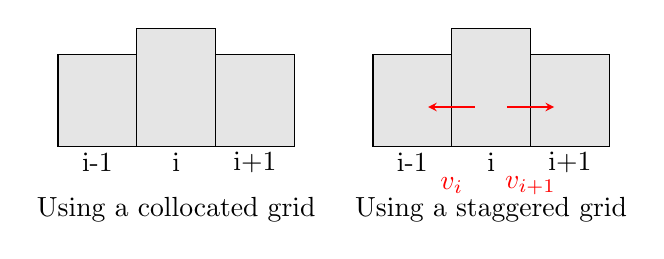
\begin{tikzpicture}
%Collocated grid
\filldraw[fill=black!10!white, draw=black] (0,0) rectangle (1,1.168);
\node[] at (0.5,-0.2) {i-1};
\filldraw[fill=black!10!white, draw=black] (1,0) rectangle (2,1.5);
\node[] at (1.5,-0.2) {i};
\filldraw[fill=black!10!white, draw=black] (2,0) rectangle (3,1.168);
\node[] at (2.5,-0.2) {i+1};
\node[] at (1.5,-0.8) {Using a collocated grid};
%Staggered grid
\filldraw[fill=black!10!white, draw=black] (4,0) rectangle (5,1.168);
\node[] at (4.5,-0.2) {i-1};
\filldraw[fill=black!10!white, draw=black] (5,0) rectangle (6,1.5);
\node[] at (5.5,-0.2) {i};
\filldraw[fill=black!10!white, draw=black] (6,0) rectangle (7,1.168);
\node[] at (6.5,-0.2) {i+1};
\draw [red, stealth-] (4.7, 0.5) -- (5.3, 0.5);
\draw [red, -stealth] (5.7, 0.5) -- (6.3, 0.5);
\node[red] at (5,-0.5) {\(v_{i}\)};
\node[red] at (6,-0.5) {\(v_{i+1}\)};
\node[] at (5.5,-0.8) {Using a staggered grid};
\end{tikzpicture} \caption{Collocated and staggered grids} \label{Odd-even decoupling} \end{figure}
%Odd-even decoupling
The Finite Difference Method calculates the pressure and velocity at discrete grid points. We can choose ourselves which variables will be calculated at which points. It would be the most easy to store all variables at every point. Such a grid is called a collocated grid\cite{Staggered grid}. However, as figure \ref{Odd-even decoupling} shows, there will be no fluid flow between cell i-1 and i and cell i and i+1 when the pressure in cells i-1 and i+1 is equal in such a grid. This phenomenon is called odd-even decoupling and happens because the derivative in cell i will be zero\cite{Staggered grid}. It is called so because information from odd and even cells are not combined properly\cite{Staggered grid}. To solve that problem we will use a staggered grid, such as in the right side of figure \ref{Odd-even decoupling}. A staggered grid consists of cells. The pressure is stored in the cell center and the velocities in the cell edges that are perpendicular to them\cite{Staggered grid}. As one can see, the derivatives will not be zero anymore, since the flow between two cells will not depend on the pressure in other cells anymore.
\newpage
\subsection{Boundary conditions and walls}
\begin{figure}[ht]
% body of the figure
\centering
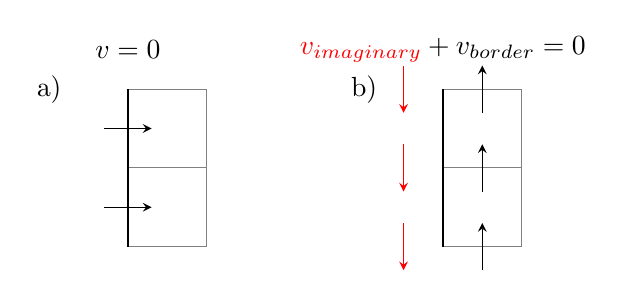
\begin{tikzpicture}
\draw[step=1cm,gray,thin] (0,0) grid (1,2);
\draw [thick] (0,0) -- (0, 2);
\draw [-stealth] (-0.3,0.5) -- (0.3, 0.5); 
\draw [-stealth] (-0.3,1.5) -- (0.3, 1.5);
\node[] at (0, 2.5) {$v=0$};
\node[] at (-1, 2) {a)};

\draw[step=1cm,gray,thin] (4,0) grid (5,2);
\draw [thick] (4,0) -- (4, 2);
\draw [-stealth] (4.5,-0.3) -- (4.5, 0.3); 
\draw [-stealth] (4.5,0.7) -- (4.5, 1.3);
\draw [-stealth] (4.5,1.7) -- (4.5, 2.3);
\node[] at (3, 2) {b)};

\draw [stealth-, red] (3.5,-0.3) -- (3.5, 0.3); 
\draw [stealth-, red] (3.5,0.7) -- (3.5, 1.3);
\draw [stealth-, red] (3.5,1.7) -- (3.5, 2.3);

\node[] at (4, 2.5) {$\textcolor{red}{v_{imaginary}}+v_{border}=0$};

\end{tikzpicture}

\caption{Wall boundary conditions} \label{wall boundary conditions}
\end{figure}

The water container is surrounded by walls on all sides.  We will use a no-slip boundary conditions at the walls, as discussed in paragraph \ref{no-slip boundary condition}\cite{MAC}. This means the velocities of the water at the wall will be equal to the velocity of the wall. The wall velocity is always zero, so the velocity of the water is zero at points on the wall. Therefore, all velocity components should be zero for wall points\cite{MAC}. Unfortunately, as can be seen in figure \ref{wall boundary conditions}.a only the velocity perpendicular to the wall has points that are at the wall. However, by using an imaginary velocity outside the box we can obtain the velocity at the wall using the average\cite{MAC}:
\[v_{wall}=\frac{v_{imaginary}+v_{border}}{2}\]
Here v is parallel to the wall(so not necessarily in the y-direction), \(v_{wall}\) is the velocity at a wall point, \(v_{border}\) is the velocity that is closest to the certain wall point and \(v_{imaginary}\) is the imaginary velocity. We can modify the formula to obtain \(v_{imaginary}\) quite easily:
\[\begin{split}
&v_{wall}=0\\
&=>\frac{v_{imaginary}+v_{border}}{2}=0\\
&=>v_{imaginary}+v_{border}=0\\
&=>v_{imaginary}=-v_{border}\\
\end{split}\]
Because of the imaginary velocity grid points, we will have to make the grid larger in some directions.\\ \\

In short, we have the following boundary conditions: \\
1) The velocities on the edge of the box that are perpendicular to the box are zero.\\
2) The imaginary velocities are equal to the inverse of the velocities opposite of the wall.

\newpage
\subsection{The sizes of the grids}
\begin{figure}[ht]
\centering
% body of the figure
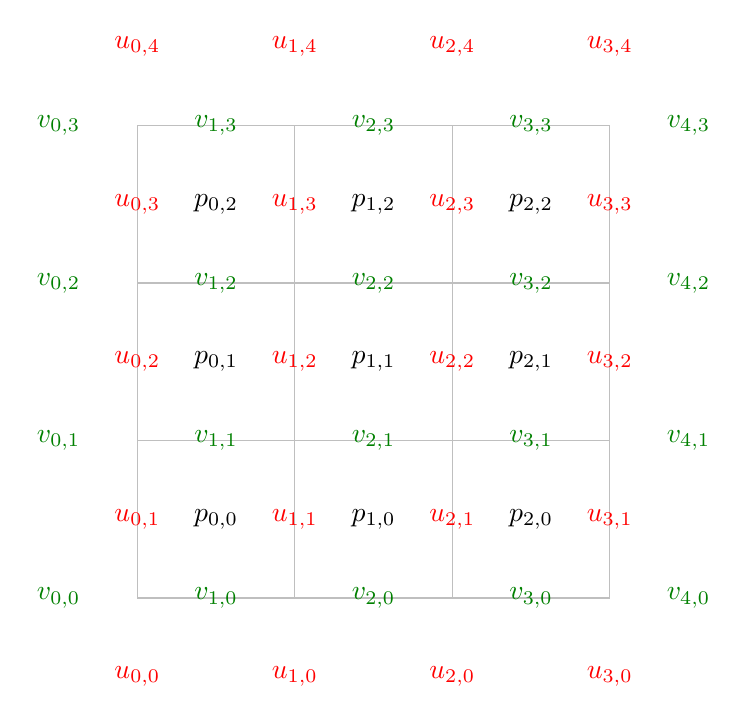
\begin{tikzpicture}
\draw[step=2cm,gray!50!white,thin] (0,0) grid (6,6);

\foreach \x in {0,1,2}
  \foreach \y in {0,1,2}
    \draw (2* \x cm + 1cm, 2* \y cm + 1cm) node[] {$p_{\x, \y}$};

\foreach \x in {0,1,2,3}
  \foreach \y in {0,1,2, 3, 4}
    \draw[red] (2* \x cm, 2* \y cm - 1cm) node[] {$u_{\x, \y}$};

\foreach \x in {0,1,2, 3, 4}
  \foreach \y in {0,1,2,3}
    \draw[green!50!black] (2* \x cm -1cm, 2* \y cm ) node[] {$v_{\x, \y}$};
    

\end{tikzpicture}
\caption{A 3*3 pressure grid}
\label{grid sizes}
\end{figure}

If we were using a collocated grid we would store our data in an array with the desired dimensions. However, we are using a staggered grid. This complicates the grid sizes a lot. We will have to use three seperate grids for velocity with different sizes and another grid for the pressure. Let u, v and w denote the velocities in respectively the x, y and z direction. The size of the pressure grid are m*n*o. In the directions that are orthogonal to the velocities of a velocity grid the size of that grid will be the size of the pressure grid plus one. We have illustrated this in figure \ref{grid sizes}. The size of the grid in the dimension that is parallel to the velocities that the grid contains is the pressure grid size plus two. The sizes in those directions are that size because of the imaginary velocities we need to store.

\newpage





\subsection{Discretising the convection term and implementing the grid}
Computers can not exactly calculate the derivatives, so we will have to approximate them to solve equation \ref{NSE incompressible}. We will be using Forward Time Central Space(FTCS) for approximating the derivatives\cite{MAC}. This means we will use first order forward derivatives for time and second order central derivatives for space. We can calculate the convection terms \(u\pdv{u}{x}\), \(v\pdv{v}{y}\) and \(w\pdv{w}{x}\)  using equation \ref{taylor deriative}. In the equations below, one might notice that we have used \(\Delta x\) everywhere and have not used \(\Delta y\) or \(\Delta z\). We have done this because we set \(\Delta x = \Delta y = \Delta z\).
\[\begin{split}
  u\pdv{u}{x}=& u_{i,j,k}\frac{u_{i+1,j.k}-u_{i-1,j,k}}{2\Delta x}\\
  v\pdv{v}{y}=& v_{i,j,k}\frac{v_{i,j+1.k}-v_{i,j-1,k}}{2\Delta x}\\
  w\pdv{w}{z}=& w_{i,j,k}\frac{w_{i,j.k+1}-w_{i,j,k-1}}{2\Delta x}
\end{split}\]
However, calculating the other convection terms is more complex, because we have to estimate a velocity at point (i,j,k) of a grid which is not defined at that grid point. We can however estimate those velocities by taking the average of some nearby velocities, as in figure \ref{velocity to other grid}\cite{MAC}.
\begin{figure}[h]
\centering
% body of the figure
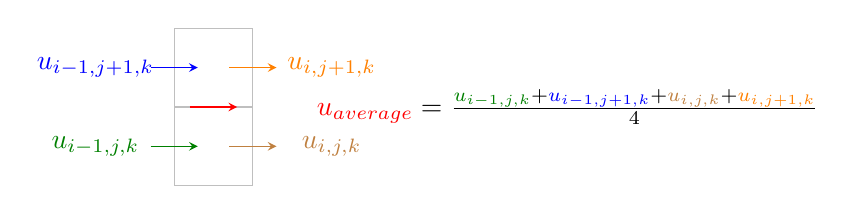
\begin{tikzpicture}
\draw[step=1cm,gray!50!white,thin] (0,0) grid (1,2);
\draw [-stealth, green!50!black] (-0.3,0.5) -- (0.3, 0.5);
\node[] at (-1, 0.5) {$\textcolor{green!50!black}{u_{i-1,j,k}}$};
\draw [-stealth, blue] (-0.3,1.5) -- (0.3, 1.5);
\node[] at (-1, 1.5) {$\textcolor{blue}{u_{i-1,j+1,k}}$};
\draw [-stealth, brown] (0.7,0.5) -- (1.3, 0.5);
\node[] at (2, 0.5) {$\textcolor{brown}{u_{i,j,k}}$};
\draw [-stealth, orange] (0.7,1.5) -- (1.3, 1.5);
\node[] at (2, 1.5) {$\textcolor{orange}{u_{i,j+1,k}}$};
\draw [-stealth, red] (0.2,1) -- (0.8, 1);
\node[] at (5, 1) {$\textcolor{red}{u_{average}}=
\frac{\textcolor{green!50!black}{u_{i-1,j,k}}+
\textcolor{blue}{u_{i-1,j+1,k}}+
\textcolor{brown}{u_{i,j,k}}+
\textcolor{orange}{u_{i,j+1,k}}}{4}
$};
\end{tikzpicture}

\caption{average of velocity} \label{velocity to other grid}
\end{figure}

\[\begin{split}
  %x velocity
  v\pdv{u}{y}&=\frac{v_{i,j-1,k}+v_{i+1,j-1,k}+v_{i,j,k}+v_{i+1,j,k}}{4}\frac{u_{i,j+1,k}-u_{i,j-1,k}}{2\Delta x}\\
  w\pdv{u}{z}&=\frac{w_{i,j,k-1}+w_{i+1,j,k-1}+w_{i,j,k}+w_{i+1,j,k}}{4}\frac{u_{i,j,k+1}-u_{i,j,k-1}}{2\Delta x}\\
  %y velocity
  u\pdv{v}{x}&=\frac{u_{i-1,j,k}+u_{i-1,j+1,k}+u_{i,j,k}+u_{i,j+1,k}}{4}\frac{v_{i+1,j,k}-v_{i-1,j,k}}{2\Delta x}\\
  w\pdv{v}{z}&=\frac{w_{i,j,k-1}+w_{i,j+1,k-1}+w_{i,j,k}+w_{i,j+1,k}}{4}\frac{v_{i,j,k+1}-v_{i,j,k-1}}{2\Delta x}\\
  %z-velocity
  u\pdv{w}{x}&=\frac{u_{i-1,j,k}+u_{i-1,j,k+1}+u_{i,j,k}+u_{i,j,k+1}}{4}\frac{w_{i+1,j,k}-w_{i-1,j,k}}{2\Delta x}\\
  v\pdv{w}{y}&=\frac{v_{i,j-1,k}+v_{i,j-1,k+1}+v_{i,j,k}+v_{i,j,k+1}}{4}\frac{w_{i,j+1,k}-w_{i,j-1,k}}{2\Delta x}\\
\end{split}
\] \label{average and partial}
We do not want to use these long equations in the code everywhere, since that would be a lot of work and unclear. Therefore, we will create a function that will calculate the partial derivative and a function that will calcute the avergage velocity at at point. To do this, we first need to create a struct that stores a velocity grid and the dimension of that grid.

\begin{lstlisting}[language=Rust, style=boxed, breaklines=true]
pub struct VelocityGrid{
    grid: Vec<Vec<Vec<f32>>>,
    dimension: usize,
}
\end{lstlisting}
As one can see, the grid is stored in a vector(Vec means vector). In Rust, a vector is an array that can have different sizes. Furthermore, the dimension of the array is stored as a usize, which basically is an integer with a maximum length that corresponds to the maximum length of an array. The values 0,1 and 2 for dimension denote the x-, y-, and z-direction respectively. To prevent the use of a lot of if-statement, we create a function that can convert the dimension number to an array for which all elements, except the element corresponding to the dimension number are zero. 
\begin{lstlisting}[language=Rust, style=boxed, breaklines=true]
//Gives you the unit vector of the dimension with the given number.
//x - 0, y - 1, z - 2
fn get_dimension(dimension_number:usize)->[usize; 3]{
    let mut dim = [0,0,0];
    dim[dimension_number]=1;
    return dim;
}
\end{lstlisting}

Next, we define the sizes of the grid, the velocity grid sizes will depend on the pressure grid sizes, so we will define the pressure grid sizes:
\begin{lstlisting}[language=Rust, style=boxed, breaklines=true]
//Grid size(e.g. number of elements in each dimension)
const PRESSUREGRIDSIZE: [usize; 3] = [10,10,10];//x,y,z
\end{lstlisting}
Now we can create a function for the second order spatial derivative.
\begin{lstlisting}[language=Rust, style=boxed, breaklines=true]
fn second_order_spatial_derivative(f:&VelocityGrid, x: usize, y:usize, z:usize, dimension_number:usize) -> f32{
    let dim= get_dimension(dimension_number);
    return (f.grid[x+dim[0]][y+dim[1]][z+dim[2]] - f.grid[x-dim[0]][y-dim[1]][z-dim[2]])/(2.0*GRIDELEMENTSCALE);
}
\end{lstlisting}
Besides that, we can now also calculate the average velocity, as in figure \ref{velocity to other grid}.
\begin{lstlisting}[language=Rust, style=boxed, breaklines=true]
//This function will retrieve the velocity of an orthogonal grid a grid point of another grid.
fn get_velocity_from_orthogonal_grid(orthogonal_grid: &VelocityGrid, x:usize, y:usize, z:usize, other_grid_dimension:usize) -> f32{
    let dim_to=get_dimension(other_grid_dimension);
    let dim_from=get_dimension(orthogonal_grid.dimension);
    return 0.25*(orthogonal_grid.grid[x-dim_from[0]][y-dim_from[1]][z-dim_from[2]]//Left down
        +orthogonal_grid.grid[x-dim_from[0]+dim_to[0]][y-dim_from[1]+dim_to[1]][z-dim_from[2]+dim_to[2]]//left up
        +orthogonal_grid.grid[x][y][z]//right down
        +orthogonal_grid.grid[x+dim_to[0]][y+dim_to[1]][z+dim_to[2]]);//right up
}
\end{lstlisting}

\newpage
\subsection{Discretising the diffusion term}
Like the convection term, the diffusion term contains no temporal terms. Of course it varies, since it terms do vary over time, but we can calculate it using information from only one timestep. We will abreviate the diffusion term of u as \(\partial _{d}u\) and the diffusion terms of v and w in a similar way\cite{MAC}. The diffusion terms of equation \ref{NSE incompressible} are\cite{MAC}:
\begin{equation}
\begin{split}
\partial _{d}u=&\eta (\pdv[2]{u}{x}+\pdv[2]{u}{y}+\pdv[2]{u}{z})\\
\partial _{d}v=&\eta (\pdv[2]{v}{x}+\pdv[2]{v}{y}+\pdv[2]{v}{z})\\
\partial _{d}w=&\eta (\pdv[2]{w}{x}+\pdv[2]{w}{y}+\pdv[2]{w}{z})\\
\end{split}
\end{equation}
We can calculate it using equation \ref{second derivative}:

\begin{lstlisting}[language=Rust, style=boxed, breaklines=true]
fn second_order_second_spatial_derivative(f: &VelocityGrid, x:usize, y:usize, z:usize, dimension_number:usize) -> f32{
    let dim = get_dimension(dimension_number);
    return(f.grid[x+dim[0]][y+dim[1]][z+dim[2]]-2.0*f.grid[x][y][z]+f.grid[x-dim[0]][y-dim[1]][z-dim[2]])/(GRIDELEMENTSCALE*GRIDELEMENTSCALE);
}
\end{lstlisting}
The sum of all three second derivatives is called the laplacian. \cite{MAC}
\begin{lstlisting}[language=Rust, style=boxed, breaklines=true]
//Laplacian velocity grid
fn laplacian(f: &VelocityGrid, x:usize, y:usize, z:usize)->f32{
    return second_order_second_spatial_derivative(f, x, y, z, 0)+second_order_second_spatial_derivative(f, x, y, z, 1)+second_order_second_spatial_derivative(f, x, y, z, 2);
}
\end{lstlisting}
So we are now able to calculate the diffusion term using:
\begin{lstlisting}[language=Rust, style=boxed, breaklines=true]
let diffusion=VISCOSITY*(laplacian(velocity_field, x, y, z));
\end{lstlisting}
We will not put this into a function already, because we do not know all the other terms yet. We will however add the constant VISCOSITY:
\begin{lstlisting}[language=Rust, style=boxed, breaklines=true]
const VISCOSITY: f32 = 0.001;//Viscosity in Pa*s.
\end{lstlisting}
\subsection{Discretising the time}
Like we expressed the diffusion terms as \(\partial _{d}\) we will express the convection terms as \(\partial _{c}\)\cite{MAC}.
\[
\begin{split}
  \partial _cu=\rho(&u\pdv{u}{x}+v\pdv{u}{y}+w\pdv{u}{z})\\
  \partial _cv=\rho(&u\pdv{v}{x}+v\pdv{v}{y}+w\pdv{v}{z})\\
  \partial _cw=\rho(&u\pdv{w}{x}+v\pdv{w}{y}+w\pdv{w}{z})
\end{split}
\]
So, we can write equation \ref{NSE incompressible} as\cite{MAC}:
\begin{equation}
\begin{split}
  \rho \pdv{u}{t} + \partial _cu=&-\pdv{p}{x}+\partial _du\\
  \rho \pdv{v}{t} + \partial _cv=&-\pdv{p}{y}+\partial _dv\\
  \rho \pdv{w}{t} + \partial _cw=&-\pdv{p}{z}+\partial _dw
\end{split}
\end{equation}\label{short NSE}
We use this notation because it is a lot shorter and As discussed previously, we will use forward time for the derivatives. Let \(a^n\) denote a in the current timestep and \(a^{n+1}\) a in the next timestep, where a is a variable. We can rewrite the above equations to: \cite{MAC}
\begin{equation}
\begin{split}
  \rho \frac{u^{n+1}-u^n}{\Delta t} + \partial _cu=&-\pdv{p^{n+1}}{x}+\partial _du\\
  \rho \frac{v^{n+1}-v^n}{\Delta t} + \partial _cv=&-\pdv{p^{n+1}}{y}+\partial _dv\\
  \rho \frac{w^{n+1}-w^n}{\Delta t} + \partial _cw=&-\pdv{p^{n+1}}{z}+\partial _dw
\end{split}
\end{equation} \label{time discretised NSE}
Unfortunately, we now have two variables for each formula: \(\frac{u^{n+1}-u^n}{\Delta t}\) and \(\pdv{p^{n+1}}{x}\), for x for instance. Therefore, we can not just solve this formula. We can however set the pressure term to the current pressure term and correct the error that is created in that way later. We will denote the velocities obtained in that way \(\tilde{u}\), \(\tilde{v}\) and \(\tilde{w}\)\cite{MAC}.
\begin{equation}
\begin{split}
  \rho \frac{\tilde{u}-u^n}{\Delta t} + \partial _cu=&-\pdv{p^{n}}{x}+\partial _du\\
  \rho \frac{\tilde{v}-v^n}{\Delta t} + \partial _cv=&-\pdv{p^{n}}{y}+\partial _dv\\
  \rho \frac{\tilde{w}-w^n}{\Delta t} + \partial _cw=&-\pdv{p^{n}}{z}+\partial _dw
\end{split}
\end{equation} \label{guess NSE}
These equations contain only one unknown variable(per equation). We can rewrite them to calculate that variable. 
\[
  \begin{split}
  \tilde{u}=u^{n}+\frac{\Delta t}{\rho}(-\pdv{p^{n}}{x}-\partial _cu +\partial _du)\\
  \tilde{v}=v^{n}+\frac{\Delta t}{\rho}(-\pdv{p^{n}}{y}-\partial _cv +\partial _dv)\\
  \tilde{w}=w^{n}+\frac{\Delta t}{\rho}(-\pdv{p^{n}}{z}-\partial _cw +\partial _dw)
  \end{split}
\]

\subsection{Drawing}
The way we decided to show the movement of the fluids is by drawing arrows in a space of three dimensions. We do this by first loading in the arrow from an OBJ file. and OBJ file is the simplest way of storing three dimensional objects. We define the center of the arrow as (0,0,0). This makes rotation and translation easier. We also make sure that by default the arrow position is up, giving us the vector $\vec{v}=(0,0,1)$. We then create multiple instances of that arrow which we multiply with a quaternion that is the cross product of the desired rotation and the neutral rotation and we set the scalar equal to the distance between the endpoints of the vectors with the origin as a starting point. finally we transform the arrow by a vector $\vec{x}=(x,y,z)$, giving us the following transformation: 
$\begin{bmatrix}
1 & 0 & 0 & 0\\
0 & 1 & 0 & 0\\
0 & 0 & 1 & 0\\
x & y & z & 1
\end{bmatrix}$. Due to the z-component in compute graphics being defined as the distance from the screen and the height as the y-component, we also need to switch the z and y-components.$\begin{bmatrix}
1 & 0 & 0 & 0\\
0 & 0 & 1 & 0\\
0 & 1 & 0 & 0\\
x & y & z & 1
\end{bmatrix}$


\newpage
%Eind PWS, start bronnenlijst
\begin{thebibliography}{3}
\bibitem{Discretization types}
\url{https://resources.pcb.cadence.com/blog/2020-cfd-simulation-types-discretization-approximation-and-algorithms}
\bibitem{What is discretization}
\url{https://www.manchestercfd.co.uk/post/what-is-discretization}
\bibitem{Difference equation}
\url{https://www.britannica.com/science/difference-equation}
\bibitem{Taylor series}
\url{https://courses.engr.illinois.edu/cs357/fa2019/assets/lectures/Lecture8-Sept19.pdf}
\bibitem{Navier_Stokes_afleiding}
\url{https://web.iit.edu/sites/web/files/departments/academic-affairs/academic-resource-center/pdfs/Navier_Stokes.pdf}
\bibitem{Fluid simulation methods}
\url{https://www.dive-solutions.de/articles/cfd-methods}
\bibitem{Lattice Boltzmann implementation}
\url{https://arxiv.org/pdf/cs/0501021.pdf}
\bibitem{Taylor series approximation}
\url{https://brilliant.org/wiki/taylor-series-approximation/}
\bibitem{quantstart FDM}
\url{https://www.quantstart.com/articles/Derivative-Approximation-via-Finite-Difference-Methods/}
\bibitem{Big O}
\url{https://math.stackexchange.com/questions/501735/why-do-we-use-big-oh-in-taylor-series}
\bibitem{Maxwell FDM}
\url{https://maxwell.ict.griffith.edu.au/jl/Chapter5.pdf}
\bibitem{Boundary Element Method}
\url{https://pure.tue.nl/ws/files/3372975/696955.pdf}
\bibitem{Finite Element Method}
\url{https://www.comsol.com/multiphysics/finite-element-method}
\bibitem{Finite Volume}
\url{https://link.springer.com/chapter/10.1007\%2F978-3-319-16874-6\_19}
\bibitem{More_FDM}
\url{http://www.fem.unicamp.br/~phoenics/SITE_PHOENICS/Apostilas/CFD-1_U\%20Michigan_Hong/Lecture13.pdf}
\bibitem{no-slip boundary condition}
\url{https://www.quora.com/What-is-the-physics-behind-no-slip-condition-in-fluid-mechanics}
\bibitem{free slip boundary condition}
\url{https://physics.stackexchange.com/questions/383096/understanding-free-slip-boundary-condition}
%Begin of Navier-Stokes
\bibitem{Navier Stokes incompressible}
\url{https://www.tec-science.com/mechanics/gases-and-liquids/derivation-of-the-navier-stokes-equations/}
\bibitem{Stresses}
\url{https://www.paramvisions.com/2021/04/what-is-normal-stress-shear-stress.html}
\bibitem{Navier Stokes compressible}
\url{http://ingforum.haninge.kth.se/armin/fluid/exer/deriv_navier_stokes.pdf}
%Neglections
\bibitem{NSE features}
\url{https://projects.iq.harvard.edu/files/ac274_2015/files/lecture2_3.pdf}
\bibitem{Viscosity}
\url{https://physics.info/viscosity/}
\bibitem{Dissipation}
\url{https://www.tec-science.com/thermodynamics/thermodynamic-processes-in-closed-systems/what-is-meant-by-dissipation-of-energy/}
\bibitem{Turbulence}
\url{https://www.simscale.com/blog/2017/12/turbulence-cfd-analysis/}
\bibitem{Steady and unsteady}
\url{http://www.nzdl.org/cgi-bin/library?e=d-00000-00---off-0hdl--00-0----0-10-0---0---0direct-10---4-------0-1l--11-en-50---20-about---00-0-1-00-0--4----0-0-11-10-0utfZz-8-00\&cl=CL1.11\&d=HASH011f05bf8734d88d1a080257.12.1\&gt=1}
\bibitem{NASA NSE}
\url{https://www.grc.nasa.gov/WWW/k-12/airplane/nseqs.html}
%End of Navier Stokes
%Projection method
\bibitem{Staggered grid}
\url{https://www.youtube.com/watch?v=Kf_RHzaqFBc}
\bibitem{MAC}
\url{https://www.youtube.com/watch?v=0qtvRjuTihY}
\bibitem{Vulkan}
https://vulkan-tutorial.com/
\bibitem{visual room}
\url{http://thevisualroom.com/marker_and_cell_method.html}
\end{thebibliography}
\end{document}
